\chapter{Carbonilos conjugados: Michael y Robinson}\label{ch:b2:conjugate-additions}

Los cuatro anillos de una hormona esteroidea se ensamblaron por primera vez de uno en uno, y una secuencia de
reacciones se convirtió en el método estándar para añadir un anillo: construye un anillo entero de seis eslabones, cetona
incluida, a partir de una cetona y de una pequeña cetona insaturada. Funciona porque un grupo carbonilo conjugado
con un doble enlace \ce{C=C} transmite su carácter electrófilo al extremo lejano de ese doble enlace.
Este capítulo trata de ese extremo lejano: qué nucleófilos lo atacan, por qué, y qué puede construirse con él.

\begin{recall}
\Cref{ch:b2:enolates-aldol}: \omterm{def:b2:enolates-aldol:enolate}{enolatos}, \omterm{def:b2:enolates-aldol:aldol}{condensación aldólica}. \Cref{ch:b2:frontier-orbitals}: \omterm{def:b2:frontier-orbitals:control}{control de carga}
y \omterm{def:b2:frontier-orbitals:control}{control orbital}, reactivos duros y blandos. \Cref{ch:b2:huckel}: orbitales de Hückel y cargas $\pi$.
El volumen del primer año: reactivos de Grignard e hidruros, control cinético y termodinámico, sistemas
conjugados.
\end{recall}

\section{Dos centros electrófilos}

\begin{definition}[Compuestos carbonílicos $\alpha,\beta$-insaturados]\label{def:b2:conjugate-additions:enone}
Un \emph{compuesto carbonílico $\alpha,\beta$-insaturado}\index{compuesto carbonilico alfa,beta-insaturado@compuesto carbonílico $\alpha,\beta$-insaturado}
tiene un doble enlace \ce{C=C} entre los carbonos $\alpha$
y $\beta$ de un compuesto carbonílico, conjugado con el \ce{C=O}: una enona (cetona), un enal
(aldehído), un éster o un \omterm{def:b2:amines:nitrile}{nitrilo} insaturados. Los más sencillos son el propenal \ce{CH2=CHCHO} y la
but-3-en-2-ona \ce{CH2=CHCOCH3} (metil vinil cetona).
\end{definition}

\begin{omfigure}
\setchemfig{atom sep=1.9em}
\schemestart
\chemfig{H_2C=CH-CH=O}
\arrow{<->}
\chemfig{H_2C=CH-\chemabove{C}{\scriptstyle +}H-\chemabove{O}{\scriptstyle -}}
\arrow{<->}
\chemfig{\chemabove{C}{\scriptstyle +}H_2-CH=CH-\chemabove{O}{\scriptstyle -}}
\schemestop
\par\medskip

\begin{tikzpicture}
\begin{axis}[ybar, width=0.47\linewidth, height=4.6cm, ymin=-0.6, ymax=0.4,
  xtick={1,2,3,4}, xticklabels={C$\beta$,C$\alpha$,C(O),O}, axis x line=bottom, axis y line=left,
  extra y ticks={0}, extra y tick style={grid=major, grid style={black!50}}, enlarge x limits=0.15,
  tick label style={font=\scriptsize}, ylabel={carga $\pi$}, label style={font=\small},
  title={\small cargas $\pi$ del propenal}, bar width=8pt]
\addplot[fill=omDef!50, draw=omDef] table[x=atom, y=q] {figdata/out/bachelor-2-huckel-d.dat};
\end{axis}
\end{tikzpicture}\hfill
\begin{tikzpicture}
\begin{axis}[ybar, width=0.47\linewidth, height=4.6cm, ymin=-0.8, ymax=0.8,
  xtick={1,2,3,4}, xticklabels={C$\beta$,C$\alpha$,C(O),O}, axis x line=bottom, axis y line=left,
  extra y ticks={0}, extra y tick style={grid=major, grid style={black!50}}, enlarge x limits=0.15,
  tick label style={font=\scriptsize}, ylabel={coeficiente}, label style={font=\small},
  title={\small LUMO del propenal}, bar width=8pt]
\addplot[fill=omThm!45, draw=omThm] table[x=atom, y=c] {figdata/out/bachelor-2-huckel-d.dat};
\end{axis}
\end{tikzpicture}

{\small El propenal. Arriba: sus tres estructuras de resonancia; las dos últimas ponen una carga positiva sobre el
carbono carbonílico y sobre el carbono $\beta$. Abajo: el modelo de Hückel del
\cref{ch:b2:frontier-orbitals} ($\alpha_{\ce{O}} = \alpha + \beta$, $\beta_{\ce{CO}} = \beta$; un modelo).
La mayor carga positiva está sobre el carbono carbonílico (+0.33, frente a +0.23 sobre el carbono $\beta$); el
mayor coeficiente del \omterm{def:b2:frontier-orbitals:frontier}{LUMO} está sobre el carbono $\beta$ (0.66, frente a $-0.58$).}
\end{omfigure}

\begin{proposition}[Dos centros]\label{prop:b2:conjugate-additions:two-sites}
En un compuesto carbonílico $\alpha,\beta$-insaturado, tanto el carbono carbonílico como el carbono $\beta$ son
electrófilos. El carbono carbonílico lleva la mayor carga positiva; el carbono $\beta$ lleva el
mayor coeficiente en el \omterm{def:b2:frontier-orbitals:frontier}{LUMO}.
\end{proposition}

\begin{proof}[Argumento]
Las estructuras de resonancia sitúan una carga positiva sobre el carbono carbonílico y, a través del \ce{C=C}, sobre
el carbono $\beta$; el carbono $\alpha$ nunca es positivo. El modelo de Hückel del propenal lo hace
cuantitativo: sumando $2c^2$ sobre los dos orbitales $\pi$ ocupados se obtienen las cargas $\pi$
(\cref{def:b2:huckel:indices}) $+0.33$ sobre el carbono carbonílico, $+0.23$ sobre el carbono $\beta$, $-0.03$
sobre el carbono $\alpha$ y $-0.53$ sobre el oxígeno. El \omterm{def:b2:frontier-orbitals:frontier}{LUMO}, el orbital que recibe los electrones del nucleófilo,
es máximo en el carbono $\beta$. Los dos centros responden, pues, a los dos tipos de control
de la \cref{def:b2:frontier-orbitals:control}.
% figdata: bachelor-2/huckel.py part d
\end{proof}

\section{Adición 1,2 o adición conjugada}

\begin{definition}[Modos de adición]\label{def:b2:conjugate-additions:addition-modes}
Un nucleófilo que se adiciona al carbono carbonílico de un compuesto carbonílico $\alpha,\beta$-insaturado da una
\emph{adición 1,2}\index{adicion 1,2@adición 1,2} (contando desde el oxígeno): un alcóxido alílico y luego un
alcohol. Un nucleófilo que se adiciona al carbono $\beta$ da una \emph{adición conjugada}\index{adicion conjugada@adición conjugada}
(o adición 1,4): un \omterm{def:b2:enolates-aldol:enolate}{enolato}, que se protona sobre el carbono para dar un compuesto carbonílico saturado
sustituido en el carbono $\beta$.
\end{definition}

\begin{omfigure}
\setchemfig{atom sep=1.9em}
\schemestart
\chemfig{*6(-=-(=O)---)}
\arrow{->[\ce{CH3Li}][luego \ce{H2O}]}[,1.4]
\chemfig{*6(-=-(-[:75]CH_3)(-[:-15]OH)---)}
\schemestop
\hspace{2.5em}
\schemestart
\chemfig{*6(-=-(=O)---)}
\arrow{->[\ce{(CH3)2CuLi}][luego \ce{H2O}]}[,1.6]
\chemfig{*6(-(-CH_3)--(=O)---)}
\schemestop
\par\vspace{6pt}

{\small La ciclohex-2-en-1-ona con dos nucleófilos metilo. El metil-litio, un \omterm{def:b2:frontier-orbitals:hard-soft}{nucleófilo duro}, se adiciona
al carbono carbonílico: 1-metilciclohex-2-en-1-ol (\omterm{def:b2:conjugate-additions:addition-modes}{adición 1,2}). El dimetilcuprato de litio, uno blando,
se adiciona al carbono $\beta$: 3-metilciclohexanona (\omterm{def:b2:conjugate-additions:addition-modes}{adición conjugada}).}
\end{omfigure}

\begin{proposition}[Qué centro]\label{prop:b2:conjugate-additions:regio}
Los \omterm{def:b2:frontier-orbitals:hard-soft}{nucleófilos duros} (organolíticos, la mayoría de los reactivos de Grignard, \ce{LiAlH4}) se adicionan sobre todo en 1,2, bajo \omterm{def:b2:frontier-orbitals:control}{control
de carga}, normalmente de forma irreversible. Los \omterm{def:b2:frontier-orbitals:hard-soft}{nucleófilos blandos} (\omterm{def:b2:conjugate-additions:cuprate}{organocupratos}, \omterm{def:b2:enolates-aldol:enolate}{enolatos} estabilizados, tiolatos,
aminas) se adicionan sobre todo en 1,4, bajo \omterm{def:b2:frontier-orbitals:control}{control orbital}; el aducto conjugado, que conserva el enlace \ce{C=O}, es
además el producto más estable.
\end{proposition}

\begin{proof}[Argumento]
Un \omterm{def:b2:frontier-orbitals:hard-soft}{nucleófilo duro}, pequeño y cargado, interacciona sobre todo a través de las cargas: va al centro más positivo,
el carbono carbonílico (\cref{prop:b2:conjugate-additions:two-sites}); su adición es rápida y
no se invierte, de modo que el producto 1,2, formado más deprisa, permanece (control cinético). Un \omterm{def:b2:frontier-orbitals:hard-soft}{nucleófilo blando},
grande y polarizable, con un \omterm{def:b2:frontier-orbitals:frontier}{HOMO} alto, interacciona sobre todo a través de los \omterm{def:b2:frontier-orbitals:frontier}{orbitales frontera}: va donde
el \omterm{def:b2:frontier-orbitals:frontier}{LUMO} es mayor, el carbono $\beta$. El producto 1,4 conserva un enlace $\pi$ \ce{C=O}, más fuerte que el
enlace $\pi$ \ce{C=C} que conserva el producto 1,2; cuando las adiciones son reversibles (cianuro, aminas,
\omterm{def:b2:enolates-aldol:enolate}{enolatos} estabilizados, alcóxidos), el equilibrio deriva por tanto hacia el aducto conjugado incluso cuando el
aducto 1,2 se formó primero (control termodinámico).
\end{proof}

\begin{method}[Predecir el modo de adición]\label{met:b2:conjugate-additions:predict-mode}
\begin{enumerate}
  \item Clasifíquese el nucleófilo: duro (\ce{RLi}, \ce{RMgX}, \ce{LiAlH4}, \ce{NaBH4} con un aldehído)
        o blando (\ce{R2CuLi}, un \omterm{def:b2:enolates-aldol:enolate}{enolato} 1,3-dicarbonílico, \ce{RS-}, \ce{R2NH}, el cianuro en equilibrio).
  \item Compruébese la reversibilidad: una adición dura irreversible da el producto 1,2; una reversible,
        con tiempo, el producto 1,4.
  \item Compruébese el impedimento: un carbono $\beta$ sustituido frena la adición 1,4; un aldehído, menos impedido
        y más reactivo en su carbonilo que una cetona, favorece la 1,2.
  \item Escríbase el \omterm{def:b2:enolates-aldol:enolate}{enolato} formado por la adición 1,4: puede protonarse, o ser atrapado por un
        electrófilo.
\end{enumerate}
\end{method}

\section{Adiciones de Michael}

\begin{definition}[Adición de Michael]\label{def:b2:conjugate-additions:michael}
Una \emph{adición de Michael}\index{adicion de Michael@adición de Michael} es la \omterm{def:b2:conjugate-additions:addition-modes}{adición conjugada} de un carbanión estabilizado,
normalmente un \omterm{def:b2:enolates-aldol:enolate}{enolato}, a un compuesto carbonílico $\alpha,\beta$-insaturado o a un alqueno pobre en electrones
semejante. El nucleófilo es el \emph{dador de Michael}\index{dador de Michael} (un compuesto 1,3-dicarbonílico, un
nitroalcano, un cianoéster); el compuesto insaturado es el \emph{aceptor de Michael}\index{aceptor de Michael}
(una enona, un enal, un éster, un \omterm{def:b2:amines:nitrile}{nitrilo} o un compuesto nitro insaturados).
\end{definition}

\begin{omfigure}
\setchemfig{atom sep=1.8em}
\schemestart
\chemfig{CH_2(-[:30]COOEt)(-[:-30]COOEt)}
\arrow{<=>[\ce{EtO-}][$-$ \ce{EtOH}]}[,1.3]
\chemfig{\chemabove{C}{\scriptstyle -}H(-[:30]COOEt)(-[:-30]COOEt)}
\+
\chemfig{H_2C=CH-C(=[2]O)-CH_3}
\schemestop

\medskip
\setchemfig{atom sep=1.6em}
\schemestart
\arrow{->[adición]}[,0.95]
\chemfig{CH(-[:150]EtOOC)(-[:210]EtOOC)-CH_2-CH=C(-[2]\chemabove{O}{\scriptstyle -})-CH_3}
\arrow{->[\ce{EtOH}][$-$ \ce{EtO-}]}[,1.1]
\chemfig{CH(-[:150]EtOOC)(-[:210]EtOOC)-CH_2-CH_2-C(=[2]O)-CH_3}
\schemestop
\par\vspace{6pt}

{\small La \omterm{def:b2:conjugate-additions:michael}{adición de Michael} del propanodioato de dietilo a la but-3-en-2-ona. El etóxido forma el \omterm{def:b2:enolates-aldol:enolate}{enolato}
estabilizado; este se adiciona al carbono $\beta$; el \omterm{def:b2:enolates-aldol:enolate}{enolato} formado toma un protón del etanol, lo que
regenera el etóxido. El producto, el (3-oxobutil)propanodioato de dietilo, es un compuesto
1,5-dicarbonílico.}
\end{omfigure}

\begin{proposition}[Mecanismo de Michael]\label{prop:b2:conjugate-additions:michael}
Una \omterm{def:b2:conjugate-additions:michael}{adición de Michael} transcurre en tres etapas (desprotonación del dador, \omterm{def:b2:conjugate-additions:addition-modes}{adición conjugada}, protonación del
nuevo \omterm{def:b2:enolates-aldol:enolate}{enolato}), y la base se regenera en la última etapa: basta una cantidad catalítica.
\end{proposition}

\begin{proof}[Argumento]
El hidrógeno $\alpha$ del dador, situado entre dos carbonilos, es ácido: $\mathrm pK_a$ de unos 13 para el
propanodioato de dietilo y de 10.7 para el 3-oxobutanoato de etilo. El etóxido (etanol, 15.9) lo arranca en gran parte, lo que
es más que suficiente. El \omterm{def:b2:enolates-aldol:enolate}{enolato} estabilizado, blando, se adiciona en 1,4
(\cref{prop:b2:conjugate-additions:regio}). El \omterm{def:b2:enolates-aldol:enolate}{enolato} formado es una base más fuerte que el \omterm{def:b2:enolates-aldol:enolate}{enolato}
del dador (está estabilizado por un carbonilo, no por dos), de modo que toma un protón del disolvente y
devuelve un etóxido por cada uno consumido. La reacción global forma un enlace $\sigma$ \ce{C-C} a partir de un
enlace $\pi$ \ce{C=C}: es favorable y, con un dador estabilizado, el aducto no revierte.
% ledger: pka:ethanol, pka:diethylmalonate, pka:acetoacetate
\end{proof}

Un aducto de Michael con una cetona del lado del dador y otra del lado del aceptor es un compuesto
1,5-dicarbonílico: los dos carbonilos están separados por cinco carbonos, contando los dos carbonos carbonílicos. Esa disposición es la
firma de una \omterm{def:b2:conjugate-additions:michael}{adición de Michael}, como el compuesto $\beta$-hidroxicarbonílico lo era de la \omterm{def:b2:enolates-aldol:aldol}{aldólica}
(\cref{met:b2:enolates-aldol:aldol-recognition}).

\section{Organocupratos}

\begin{definition}[Organocupratos]\label{def:b2:conjugate-additions:cuprate}
Un \emph{organocuprato}\index{organocuprato} \ce{R2CuLi} es un compuesto de cobre(I) que lleva dos grupos
orgánicos, preparado a partir de dos equivalentes de un organolítico y uno de un haluro de cobre(I):
\begin{equation*}
\ce{2 CH3Li + CuI -> (CH3)2CuLi + LiI}.
\end{equation*}
\end{definition}

Los \omterm{def:b2:conjugate-additions:cuprate}{organocupratos} (también llamados reactivos de Gilman) se preparan y se usan en éter a baja temperatura bajo
gas inerte, como los organolíticos de los que proceden. El cobre es menos electropositivo que el litio o el
magnesio, de modo que el enlace \ce{Cu-C} es más covalente y el carbono está menos cargado: el grupo metilo de un
cuprato es un \omterm{def:b2:frontier-orbitals:hard-soft}{nucleófilo blando}. De ahí tres usos.

\begin{itemize}
  \item \emph{\omterm{def:b2:conjugate-additions:addition-modes}{Adición conjugada}} de un grupo alquilo o arilo a una enona, que los reactivos de Grignard y los
        organolíticos no realizan limpiamente; solo se transfiere uno de los dos grupos \ce{R}.
  \item \emph{Atrapado}: el \omterm{def:b2:enolates-aldol:enolate}{enolato} formado por la \omterm{def:b2:conjugate-additions:addition-modes}{adición conjugada} puede alquilarse en su carbono
        $\alpha$, de modo que se forman dos nuevos enlaces \ce{C-C} en una sola operación.
  \item \emph{Sustitución} de haluros: $\mathrm{R_2CuLi + R'Br \to R{-}R' + RCu + LiBr}$, un acoplamiento que un
        organolítico estropearía por eliminación o intercambio.
\end{itemize}

\section{La anulación de Robinson}

\begin{definition}[Anulación]\label{def:b2:conjugate-additions:robinson}
Una \emph{anulación}\index{anulacion@anulación} construye un nuevo anillo sobre una molécula existente. La \emph{anulación de Robinson}
\index{anulacion de Robinson@anulación de Robinson} construye una ciclohex-2-en-1-ona: una \omterm{def:b2:conjugate-additions:michael}{adición de Michael} del \omterm{def:b2:enolates-aldol:enolate}{enolato} de una
cetona a una cetona $\alpha,\beta$-insaturada (típicamente la but-3-en-2-ona), seguida de una
\omterm{def:b2:enolates-aldol:aldol}{condensación aldólica} intramolecular de la 1,5-dicetona formada.
\end{definition}

\begin{omfigure}
\setchemfig{atom sep=1.8em}
\schemestart
\chemfig{[:30]*6(-(=O)-(-CH_3)-(=O)---)}
\+
\chemfig{=[:30]-[:-30](=[:-90]O)-[:30]}
\arrow{->[base][Michael]}[,1.2]
\chemfig{[:30]*6(-(=O)-(-[:40]CH_3)(-[:-30]-[:30]-[:-30](=[:-90]O)-[:30])-(=O)---)}
\schemestop

\medskip
\schemestart
\arrow{->[base][aldólica]}[,1.1]
\chemfig{[:-30]*6(---(-[:-60]OH)*6(--(=O)---)-(-[:105]CH_3)-(=O)-)}
\arrow{->[calor][$-$ \ce{H2O}]}[,1.1]
\chemfig{[:-30]*6(---*6(=-(=O)---)-(-[:105]CH_3)-(=O)-)}
\schemestop
\par\vspace{6pt}

{\small La \omterm{def:b2:conjugate-additions:robinson}{anulación de Robinson} que produce la cetona de Wieland--Miescher. El \omterm{def:b2:enolates-aldol:enolate}{enolato} de la
2-metilciclohexano-1,3-diona se adiciona a la but-3-en-2-ona (Michael): una tricetona. El \omterm{def:b2:enolates-aldol:enolate}{enolato} de la
metilcetona de la cadena lateral ataca un carbonilo del anillo (\omterm{def:b2:enolates-aldol:aldol}{aldólica} intramolecular) y cierra un anillo de seis eslabones;
la deshidratación da la enona conjugada. El grupo metilo angular está sobre el carbono compartido por los dos
anillos, el único estereocentro.}
\end{omfigure}

\begin{proposition}[Anulación de Robinson]\label{prop:b2:conjugate-additions:robinson}
Una cetona con un hidrógeno $\alpha$ y la but-3-en-2-ona, en medio básico, dan una ciclohex-2-en-1-ona en tres
etapas: \omterm{def:b2:conjugate-additions:michael}{adición de Michael}, \omterm{def:b2:enolates-aldol:aldol}{adición aldólica} intramolecular que forma un anillo de seis eslabones, y deshidratación.
El nuevo anillo contiene el antiguo carbono $\alpha$ de la cetona y su carbono carbonílico, y los cuatro
carbonos de la but-3-en-2-ona.
\end{proposition}

\begin{proof}
Síganse los átomos en la figura. El carbono \omterm{def:b2:enolates-aldol:enolate}{enolato} de la cetona (llamémoslo C$_a$) se une al carbono $\beta$
de la but-3-en-2-ona: la cadena C$_a$--\ce{CH2}--\ce{CH2}--\ce{C(=O)}--\ce{CH3} cuelga de C$_a$, y
C$_a$ sigue unido al carbono carbonílico de la cetona, C$_k$. En medio básico, la metilcetona de la cadena
forma su \omterm{def:b2:enolates-aldol:enolate}{enolato} en el \ce{CH3} terminal, que ataca a C$_k$. El anillo que se cierra cuenta C$_k$, C$_a$,
los dos \ce{CH2}, el carbono carbonílico de la cadena lateral y el antiguo carbono metílico: seis átomos, el tamaño
de anillo sin tensión, y por eso este \omterm{def:b2:enolates-aldol:enolate}{enolato}, entre los posibles, conduce a un producto estable (un
ataque del \omterm{def:b2:enolates-aldol:enolate}{enolato} del \ce{CH2} interno de la cadena cerraría un anillo de cuatro eslabones). El \omterm{def:b2:enolates-aldol:aldol}{aldol} tiene su
\ce{OH} sobre C$_k$, en $\beta$ respecto al carbonilo de la cadena; la deshidratación sitúa el \ce{C=C} entre C$_k$ y el
antiguo carbono metílico, conjugado con el carbonilo: una ciclohex-2-en-1-ona.
\end{proof}

\begin{method}[Desconectar una ciclohexenona]\label{met:b2:conjugate-additions:robinson-disconnection}
\begin{enumerate}
  \item Localícese una ciclohex-2-en-1-ona en la molécula objetivo; numérese su carbono carbonílico C1, el doble enlace
        C2=C3, y el resto del anillo hasta C6.
  \item Deshágase la deshidratación: un \ce{OH} en C3, un \ce{C-H} en C2.
  \item Deshágase la \omterm{def:b2:enolates-aldol:aldol}{aldólica}: córtese C2--C3. C3 pasa a ser un carbonilo cetónico, y C2, un grupo metilo de una
        metilcetona: una 1,5-dicetona.
  \item Deshágase la \omterm{def:b2:conjugate-additions:michael}{adición de Michael}: córtese el enlace entre C4 (el carbono $\alpha$ de la cetona de C3) y
        C5. El dador es esa cetona; el aceptor es la enona C5=C6--C1(=O)--C2, que es la
        but-3-en-2-ona cuando C5, C6 y C2 solo llevan hidrógenos.
\end{enumerate}
\end{method}

\begin{history}[La anulación, 1935]
\begin{minipage}[t]{0.18\linewidth}
\vspace{0pt}
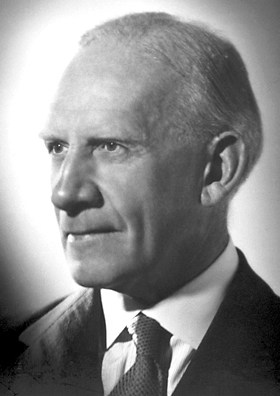
\includegraphics[width=\linewidth]{images/book3/robinson.jpg}
\end{minipage}\hfill
\begin{minipage}[t]{0.78\linewidth}
\vspace{0pt}
Robert Robinson y William Rapson publicaron la secuencia formadora de anillos en 1935, en un trabajo orientado a la
síntesis de esteroides. Los principales logros de Robinson fueron las estructuras y síntesis de alcaloides,
por los que recibió el Premio Nobel de Química de 1947. En 1950, Peter Wieland y Karl Miescher prepararon
la dicetona bicíclica del problema de este capítulo, que se convirtió en un punto de partida habitual de las síntesis de esteroides y
terpenos. (Retrato: autor desconocido, dominio público; Wikimedia Commons.)
\end{minipage}
\end{history}

\begin{safety}{\ghs[5mm]{GHS02}\,\ghs[5mm]{GHS05}\,\ghs[5mm]{GHS06}\,\ghs[5mm]{GHS07}\,\ghs[5mm]{GHS08}\,\ghs[5mm]{GHS09}}
La but-3-en-2-ona es inflamable, muy tóxica, corrosiva y peligrosa para el medio acuático, y un potente lacrimógeno; solo se manipula
en una vitrina de gases. La ciclohex-2-en-1-ona es inflamable y tóxica. Los organolíticos, los reactivos de Grignard y los
cupratos reaccionan violentamente con el agua y se manipulan bajo gas inerte.
% ledger: ghs:MVK, ghs:cyclohexenone, ghs:MeMgBr
\end{safety}

\section{Ejercicios}

\begin{exercise}[$\star$]\label{exo:b2:conjugate-additions:1}
Prevéase \omterm{def:b2:conjugate-additions:addition-modes}{adición 1,2} o 1,4 a la ciclohex-2-en-1-ona para: \ce{CH3MgBr}; \ce{(CH3)2CuLi};
\ce{C6H5SH} con un poco de base; \ce{LiAlH4}.
\end{exercise}

\begin{exercise}[$\star$]\label{exo:b2:conjugate-additions:2}
Clasifíquense como \omterm{def:b2:conjugate-additions:michael}{dador de Michael} o \omterm{def:b2:conjugate-additions:michael}{aceptor de Michael}: pentano-2,4-diona, propenonitrilo \ce{CH2=CHCN},
nitrometano, propenoato de metilo, propanodioato de dietilo, but-3-en-2-ona.
\end{exercise}

\begin{exercise}[$\star$]\label{exo:b2:conjugate-additions:3}
Escríbase la preparación del dibutilcuprato de litio a partir del 1-bromobutano, el litio y el yoduro de cobre(I).
\end{exercise}

\begin{exercise}[$\star$]\label{exo:b2:conjugate-additions:4}
Dese el producto del propanodioato de dietilo con but-3-en-2-ona y una cantidad catalítica de etóxido
de sodio, y luego el producto tras hidrólisis y calentamiento.
\end{exercise}

\begin{exercise}[$\star\star$]\label{exo:b2:conjugate-additions:5}
Propóngase una preparación de la 3-metilciclohexanona a partir de la ciclohex-2-en-1-ona, y explíquese por qué
el bromuro de metilmagnesio sería una mala elección.
\end{exercise}

\begin{exercise}[$\star\star$]\label{exo:b2:conjugate-additions:6}
El etanotiol se adiciona a la but-3-en-2-ona con una traza de trietilamina. Escríbase el mecanismo y dígase por qué el
tiolato se adiciona en 1,4.
\end{exercise}

\begin{exercise}[$\star\star$]\label{exo:b2:conjugate-additions:7}
El cianuro con la ciclohex-2-en-1-ona da, a baja temperatura y en tiempos cortos, la cianhidrina; a temperatura más
alta y en tiempos más largos, el 3-oxociclohexano-1-carbonitrilo. Explíquese mediante el control cinético y el
termodinámico.
\end{exercise}

\begin{exercise}[$\star\star$]\label{exo:b2:conjugate-additions:8}
Dese el producto de la \omterm{def:b2:conjugate-additions:robinson}{anulación de Robinson} de la 2-metilciclohexano-1,3-diona con la but-3-en-2-ona, y luego el
de la ciclohexanona con la but-3-en-2-ona.
\end{exercise}

\begin{exercise}[$\star\star$]\label{exo:b2:conjugate-additions:9}
Desconéctese la heptano-2,6-diona en un \omterm{def:b2:conjugate-additions:michael}{dador de Michael} y un \omterm{def:b2:conjugate-additions:michael}{aceptor de Michael}, y propónganse condiciones.
\end{exercise}

\begin{exercise}[$\star\star\star$]\label{exo:b2:conjugate-additions:10}
Una \omterm{def:b2:enolates-aldol:aldol}{adición aldólica} simple se invierte fácilmente en medio básico; el aducto de Michael del propanodioato de dietilo y la
but-3-en-2-ona, no. Explíquese con los enlaces formados y rotos y con la acidez del producto.
\end{exercise}

\begin{exercise}[$\star\star\star$]\label{exo:b2:conjugate-additions:11}
El propanodioato de dietilo con dos equivalentes de propenoato de metilo y una base catalítica da un producto
sin ningún \ce{C-H} entre sus dos grupos éster. Dibújese y explíquese.
\end{exercise}

\begin{exercise}[$\star\star\star$]\label{exo:b2:conjugate-additions:12}
La 2-metilciclohexanona y la but-3-en-2-ona pueden reaccionar en una \omterm{def:b2:conjugate-additions:robinson}{anulación de Robinson} a través de uno u otro \omterm{def:b2:enolates-aldol:enolate}{enolato}.
Dibújense ambos productos y dígase qué condiciones favorecen el que tiene el grupo metilo en el carbono
de fusión de los anillos.
\end{exercise}

\section{Problema: la cetona de Wieland--Miescher}

\begin{problem}[{Problema de fin de semana --- el dador ácido, el aducto de Michael, la aldólica intramolecular y
su deshidratación, el estereocentro y el balance de materia de una preparación}]
\label{pb:b2:conjugate-additions:1}
Preparación (datos de ejercicio): \qty{10.0}{g} de 2-metilciclohexano-1,3-diona reaccionan con un ligero exceso
de but-3-en-2-ona y una base catalítica (\omterm{def:b2:conjugate-additions:michael}{adición de Michael}); la tricetona se cicla después con una
\omterm{def:b2:amines:class}{amina secundaria} y un ácido (\omterm{def:b2:enolates-aldol:aldol}{aldólica}, deshidratación). Rendimiento global: 70~\%. La ciclohexano-1,3-diona de referencia
tiene $\mathrm pK_a = 5.3$ en agua. Masas molares (\unit{g/mol}): C 12.011, H 1.008, O 15.999.
% ledger: pka:cyclohexanedione, aw:C, aw:H, aw:O, ghs:methylcyclohexanedione, ghs:MVK

\medskip
\noindent\textbf{Parte I --- El dador.}
\begin{enumerate}
  \item Dibújese la 2-metilciclohexano-1,3-diona y señálese su hidrógeno más ácido.
  \item ¿Por qué ese hidrógeno es mucho más ácido que los hidrógenos $\alpha$ de la ciclohexanona?
  \item Dibújense las tres estructuras de resonancia de su \omterm{def:b2:enolates-aldol:enolate}{enolato}.
  \item ¿Es el hidróxido o el etóxido lo bastante fuerte para formar por completo este \omterm{def:b2:enolates-aldol:enolate}{enolato}? Úsese el $\mathrm pK_a$.
  \item Escríbase el \omterm{def:b2:enolates-aldol:tautomerism}{enol} de la diona en el que interviene C2, y dígase por qué el grupo metilo de C2 no
        lo impide.
  \item ¿Es este \omterm{def:b2:enolates-aldol:enolate}{enolato} duro o blando? ¿Qué centro de la but-3-en-2-ona atacará?
\end{enumerate}

\medskip
\noindent\textbf{Parte II --- El aducto de Michael.}
\begin{enumerate}[resume]
  \item Escríbase la \omterm{def:b2:conjugate-additions:michael}{adición de Michael} y nómbrese la tricetona formada.
  \item ¿Por qué solo se necesita una cantidad catalítica de base?
  \item ¿Por qué el nuevo enlace se forma en el C2 de la diona y no en su oxígeno?
  \item ¿Cuántos carbonos cuaternarios tiene la tricetona?
  \item Identifíquese la relación 1,5-dicarbonílica en la tricetona.
  \item ¿Por qué se usa un ligero exceso de but-3-en-2-ona, y por qué solo ligero?
\end{enumerate}

\medskip
\noindent\textbf{Parte III --- El cierre del anillo.}
\begin{enumerate}[resume]
  \item Enumérense los carbonos de la tricetona que llevan hidrógenos $\alpha$.
  \item ¿Qué \omterm{def:b2:enolates-aldol:enolate}{enolato}, atacando a qué carbonilo, cierra un anillo de seis eslabones?
  \item ¿Qué otros cierres de anillo podrían intentarse, y por qué no dan el producto?
  \item Escríbanse el \omterm{def:b2:enolates-aldol:aldol}{aldol} formado y la deshidratación que le sigue.
  \item ¿Por qué es fácil la deshidratación?
  \item Nómbrense los grupos funcionales de la cetona de Wieland--Miescher.
\end{enumerate}

\medskip
\noindent\textbf{Parte IV --- Estereoquímica y balance de materia.}
\begin{enumerate}[resume]
  \item ¿Qué carbono del producto es un estereocentro?
  \item ¿Es ópticamente activo el producto de esta preparación? Explíquese.
  \item Calcúlense las masas molares de la diona, de la but-3-en-2-ona y del producto
        \ce{C11H14O2}.
  \item Escríbase la ecuación global y compruébese con las fórmulas.
  \item Calcúlese la cantidad de diona utilizada.
  \item Indíquese la masa de cetona de Wieland--Miescher obtenida con un rendimiento global del 70~\%.
\end{enumerate}
\end{problem}
